\documentclass{article}

\usepackage{graphicx}
\graphicspath{{./images/}}

\title{Political Polarization via Bayesian Updating}
\author{Emmet Hall-Hoffarth and Afonso Rodrigues}
\date{\today}

\begin{document}
\maketitle
    
\section{Model}

At $t=0$ a set $C$ of $n$ agents start with and $(h \times 1)$ vector of prior beliefs over a set of $h$ issues which together form the $(n \times h)$ matrix $\pi_0$. At each time step $t > 1$ every agent will simultaniously update their beliefs according to the following procedure. Consider, without loss of generality, the case of agent 0. At the beginning of the period agent 0 will select "consideration set"; a subset of other agents $c \in C$ of size $|c|$ with whom to update their beliefs. Other agents are selected into $c$ without replacement with a probability inversely proportional to their distance in views to agent 0 (in l2-norm) and proportional to the l2-norm of that agent's belief vector, as in equation (\ref{consideration_prob}):

\begin{equation}
    P_0(i \in c) \propto \frac{{||\pi_i||}_2^\epsilon}{{||\pi_i - \pi_0||}_2^2}
    \label{consideration_prob}
\end{equation}

Where $\epsilon$ is an "extreme bias" parameter. This model embodies two mechanisms. Firstly, agents are more likely to choose other agents with similar views in their consideration set. This probability updates at every time $t$, so it captures the idea that agents may endogenously choose the views that they are exposed to, for example, on social media. Secondly, agents are more likely to consider the views of agents who lie further from the centre. We call this "extreme bias." Intuitively, this reflects the incentive of media organizations to report on controversial topics or views because they generate more viewer engagement. The relative strength of these effects depends on the parameter $\epsilon$.

Having chosen a consideration set, agent 0 now applies a simple updating rule: they update their belief in period $t+1$ to be the geometric mean of their prior beliefs and the mean of their consideration set. The equation for this is shown in (\ref{updating_rule}):

\begin{equation}
    \pi_{0, t+1} = \pi_{0, t} + \frac{\pi_{0, t} - \overline{\pi_{c, t}}}{2}
    \label{updating_rule}
\end{equation}

\section{Possible Extensions}

\begin{itemize}
    \item Not all agents update at every step (stochastic updating).
    \item Some proportion of agents are re-randomized every period (i.e. due to birth and death) (already implemented in code)
    \item Allow agents to have heterogeneous selection and updating rules.
    \item Consider the effect of high dimensions ($h$) and extreme bias ($\epsilon$) on the observed amount of polarization 
    \item Find a metric to quantify polarization.
\end{itemize}

\section{Results}
We simulate the model over $50$ iterations with the following parameters:

\begin{itemize}
    \item $n = 500$
    \item $|c|$ = 10
    \item $h = 2$
    \item $\epsilon = 1.5$ 
\end{itemize}

We obtain the following results over 50 iterations (each image is shown 10 iterations after the last):

\begin{center}

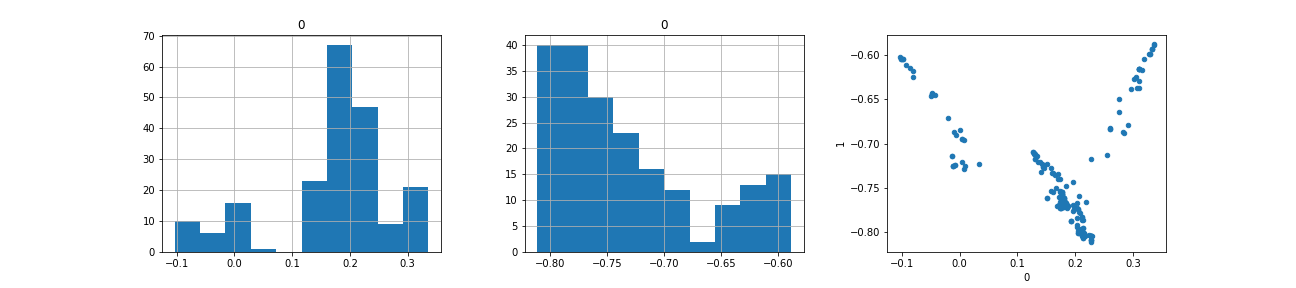
\includegraphics[width=\linewidth]{200_10_0_2_11.png}
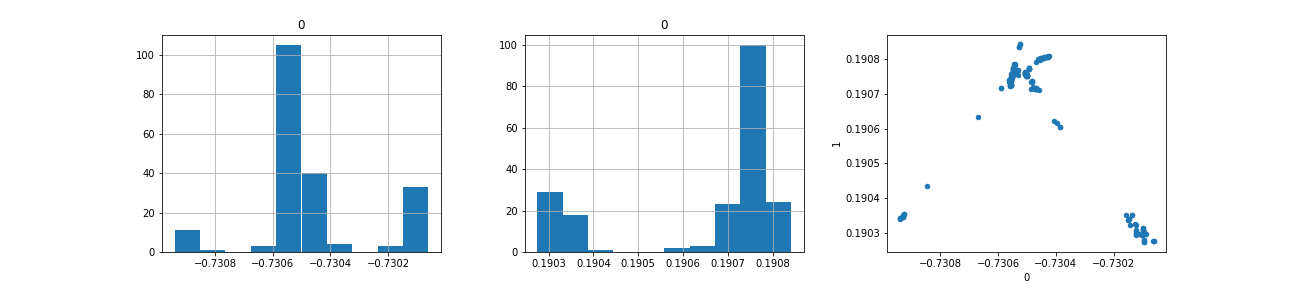
\includegraphics[width=\linewidth]{200_10_0_2_21.png}
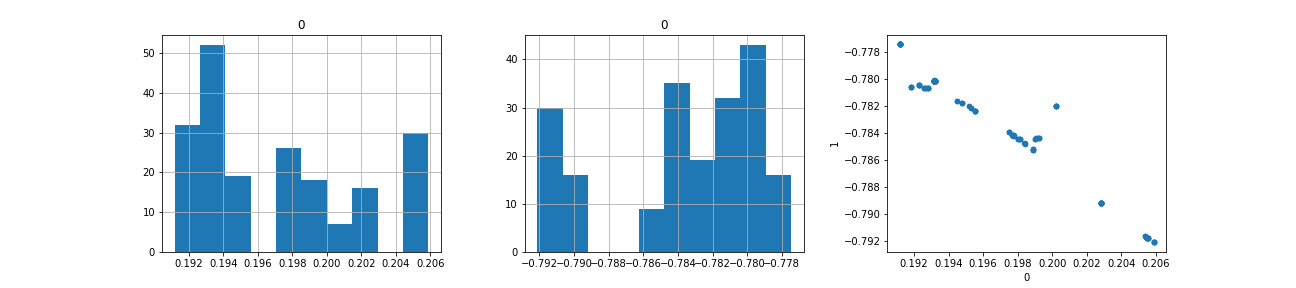
\includegraphics[width=\linewidth]{200_10_0_2_31.png}
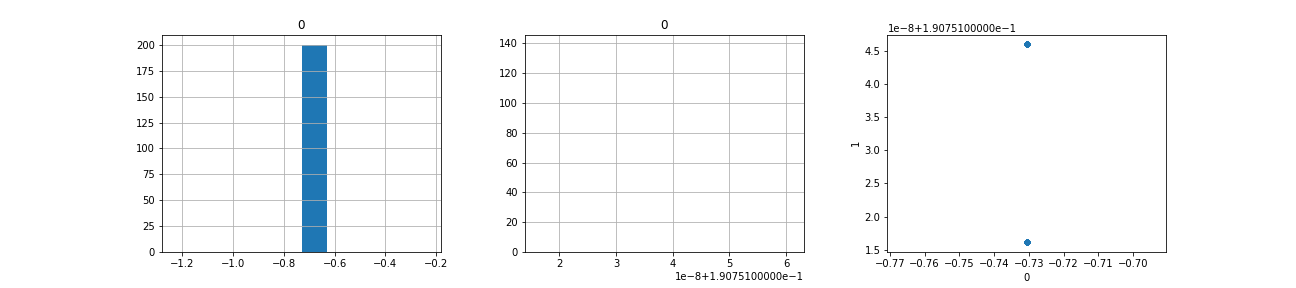
\includegraphics[width=\linewidth]{200_10_0_2_41.png}
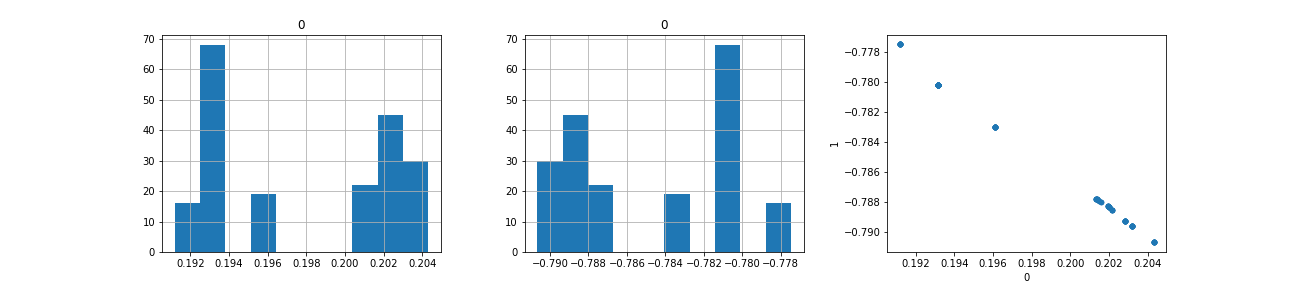
\includegraphics[width=\linewidth]{200_10_0_2_51.png}
    
\end{center}


\end{document}